\documentclass[hidelinks, 12pt,letterpaper]{article}
%%%%%%%%%%%%%%%%%%%%%%%%%%%%%%%%%%%%%%%%%%%%%%%%%%%%%%%%%%%%%%%%%%%%%%%%%%%%%%%%%%%%%%%%%%%%%%%%%%%%%%%%%%%%%%%%%%%%%%%%%%%%
\usepackage{amsmath}
%\usepackage{graphicx,fancyheadings}
\usepackage{fancyhdr}
\pagestyle{fancy}
\usepackage{graphics}
\usepackage{amssymb}
\usepackage{verbatim}
\usepackage{setspace}
\usepackage{ulem} 

\usepackage{amssymb}
\usepackage{graphicx}
\usepackage{amsmath}
\usepackage{verbatim}
\usepackage{setspace}
\usepackage{ulem}
\usepackage{textpos}
\usepackage{changepage}
\usepackage{url}
\usepackage{hyperref}

\usepackage{color}
\usepackage{xcolor}


%\renewcommand{\sout}[1]{}
%\renewcommand{\bf}{}

\usepackage[round]{natbib}
% \usepackage[backend=biber,style=apa,autocite=inline]{biblatex} \DeclareLanguageMapping{english}{english-apa}
% \addbibresource{./sshrc2023shipping.bib}


%\lhead{} \chead{} \cfoot{}
\renewcommand{\headrulewidth}{0pt}
\renewcommand{\footrulewidth}{0pt}
\renewcommand{\baselinestretch}{1.1}
%\textheight 8in \textwidth 6in \oddsidemargin 0.15in
%\evensidemargin 0in \headheight 14.5pt \headwidth 6in \parskip 4pt

\pagestyle {empty}

\setlength{\topmargin}{0.0cm} \setlength{\headheight}{0cm}
\setlength{\headsep}{0.3cm} \setlength{\topskip}{0cm}
\setlength{\textheight}{22.5cm} \setlength{\textwidth}{16.6cm}
\setlength{\oddsidemargin}{0cm} \setlength{\evensidemargin}{0cm}
\setlength{\footskip}{0.5cm}
\newcommand{\indep}{\perp \!\!\! \perp}


\newcommand{\Red}{\color{red}}
\newcommand{\Blue}{\color{blue}}
\newcommand{\ve}{\varepsilon}

\def\bs{\boldsymbol}

%\setlength{\topmargin}{-0.2cm} \setlength{\headheight}{0cm}
%\setlength{\headsep}{0.3cm} \setlength{\topskip}{0cm}
%\setlength{\textheight}{22cm} \setlength{\textwidth}{16.2cm}
%\setlength{\oddsidemargin}{0cm} \setlength{\evensidemargin}{0cm}
%\setlength{\footskip}{1cm}

\usepackage[letterpaper]{geometry}

 \rhead{Hiroyuki Kasahara \hspace{-1.7cm} }
 %\lfoot{}
 \cfoot{\thepage \hspace{-2cm}}



%\setcounter{page}{10}

\begin{document}
\bibliographystyle{asa}

% Challenge—The aim and importance of the endeavour (40\%):
% \begin{itemize}
%   \item originality, significance and expected contribution to knowledge;
%   \item appropriateness of the literature review;
%   \item appropriateness of the theoretical approach or framework;
%   \item appropriateness of the methods/approach;
%   \item quality of training and mentoring to be provided to students, emerging scholars and other highly qualified personnel, and opportunities for them to contribute; and
%   \item potential for the project results to have influence and impact within and/or beyond the social sciences and humanities research community.
% \end{itemize}
    
% Feasibility—The plan to achieve excellence (20\%):
% \begin{itemize}
%   \item appropriateness of the proposed timeline, and probability that the objectives will be met;
% \end{itemize}

\begin{center}
\textbf{Detailed Description of Proposed Research: }\vspace{-0.25cm}
\end{center}

\noindent \textbf{Project: Quantifying the response of maritime shipping CO$_2$ emissions to demand shocks} 
\smallskip 

\noindent \textbf{Objective:} To estimate the elasticity of CO$_2$ emissions from maritime shipping with respect to international trade using the COVID pandemic demand shock as a source of significant variation.
\smallskip 

\noindent \textbf{Context:} 
\textbf{Overview}
Global trade is intricately linked with maritime shipping, which carries over 80\% of the volume of all traded goods and around 70\% of their value \citep{unctad2017review}. 
% The importance of the shipping industry has become particularly apparent in recent years as disruptions ranging from the blockage of the Suez Canal to widespread COVID-related port slowdowns have snarled supply chains world-wide.
At the same time, maritime ships contribute roughly 3\% of global CO$_2$ emissions, roughly equal to the total emissions of Germany \citep*{faber2020fourth}. These emissions lie outside the scope of national emissions tallies, and fall instead under the jurisdiction the International Maritime Organization (IMO), which has set a target of a 50\% reduction by 2050.
\textcolor{blue}{mention difficulty of decarbonization?}
The stringency of abatement actions required to meet this goal clearly depends on the how trade will evolve over the coming decades. A continuation of the trend of increasing trade would make this goal much more difficult to hit, while a reversion to more protectionist policies would ease the challenge. Faced with this uncertainty, the IMO and its consituent countries are nevertheless developing and implementing policies to reduce shipping emissions, with new efficiency regulations being phased in this year. We aim to provide new quantitative evidence of the relationship between international trade and maritime shipping emissions in order to better inform policy makers. To do so, we will exploit the large variation in demand for shipping that resulted from the COVID pandemic.

The three largest sectors of maritime shipping, jointly accounting for over half of maritime emissions, are containerships, bulk carriers, and tankers. These ships transport, respectively,  containerized goods (often manufactured goods), dry bulk goods (e.g. coal, ores, grains), and bulk liquids (primarily oil). As such, they contribute to diverse links of the overall supply chain and are impacted differently by fluctuations in trade. Furthermore, each sector has distinct market characteristics. For example, containerships typically operate with fixed routes and schedules, while bulk carriers tend to operate much more flexibly. Ownership structures reflect these differences as well, with the containership sector being highly concentrated and the bulk carrier sector highly \textit{un}concentrated.

Despite their differences, the various sectors share some common mechanisms by which they adjust to demand. Because new ships cost tens to hundreds of millions of dollars, last for over 25 years, and take 2-5 years to build, adjustments in fleet capacity are slow to occur (see for example \citet{kalouptsidi2014time}). On shorter time horizons, shipping supply adjusts to changing levels of demand primarily through a combination of changing travel speed and temporarily idling ships, though quantifying these adjustments is an active area of research (see \citet*{adland2018dynamic, ollila2022effect,assmann2015missing}). CO$_2$ emissions are directly related to fuel consumption, which depends non-linearly on speed, meaning that the short run elasticity of emissions to demand may be quite large. 

Quantifying this elasticity is challenging for a number of reasons. First, a ship's fuel consumption depends on various factors, including its size and age (newer and larger ships tend to be more efficient) and the existing fleet is extremely heterogeneous. As an illustration, \autoref{fig:distribution} shows the existing fleet distribution for bulk carriers below 100,000 DWT in size (this excludes the largest classes up to just over 400,000 DWT). As such, ships adapt differently and which ships change speed or idle is important for determining overall emissions.

\begin{figure}[h]
  \centering
  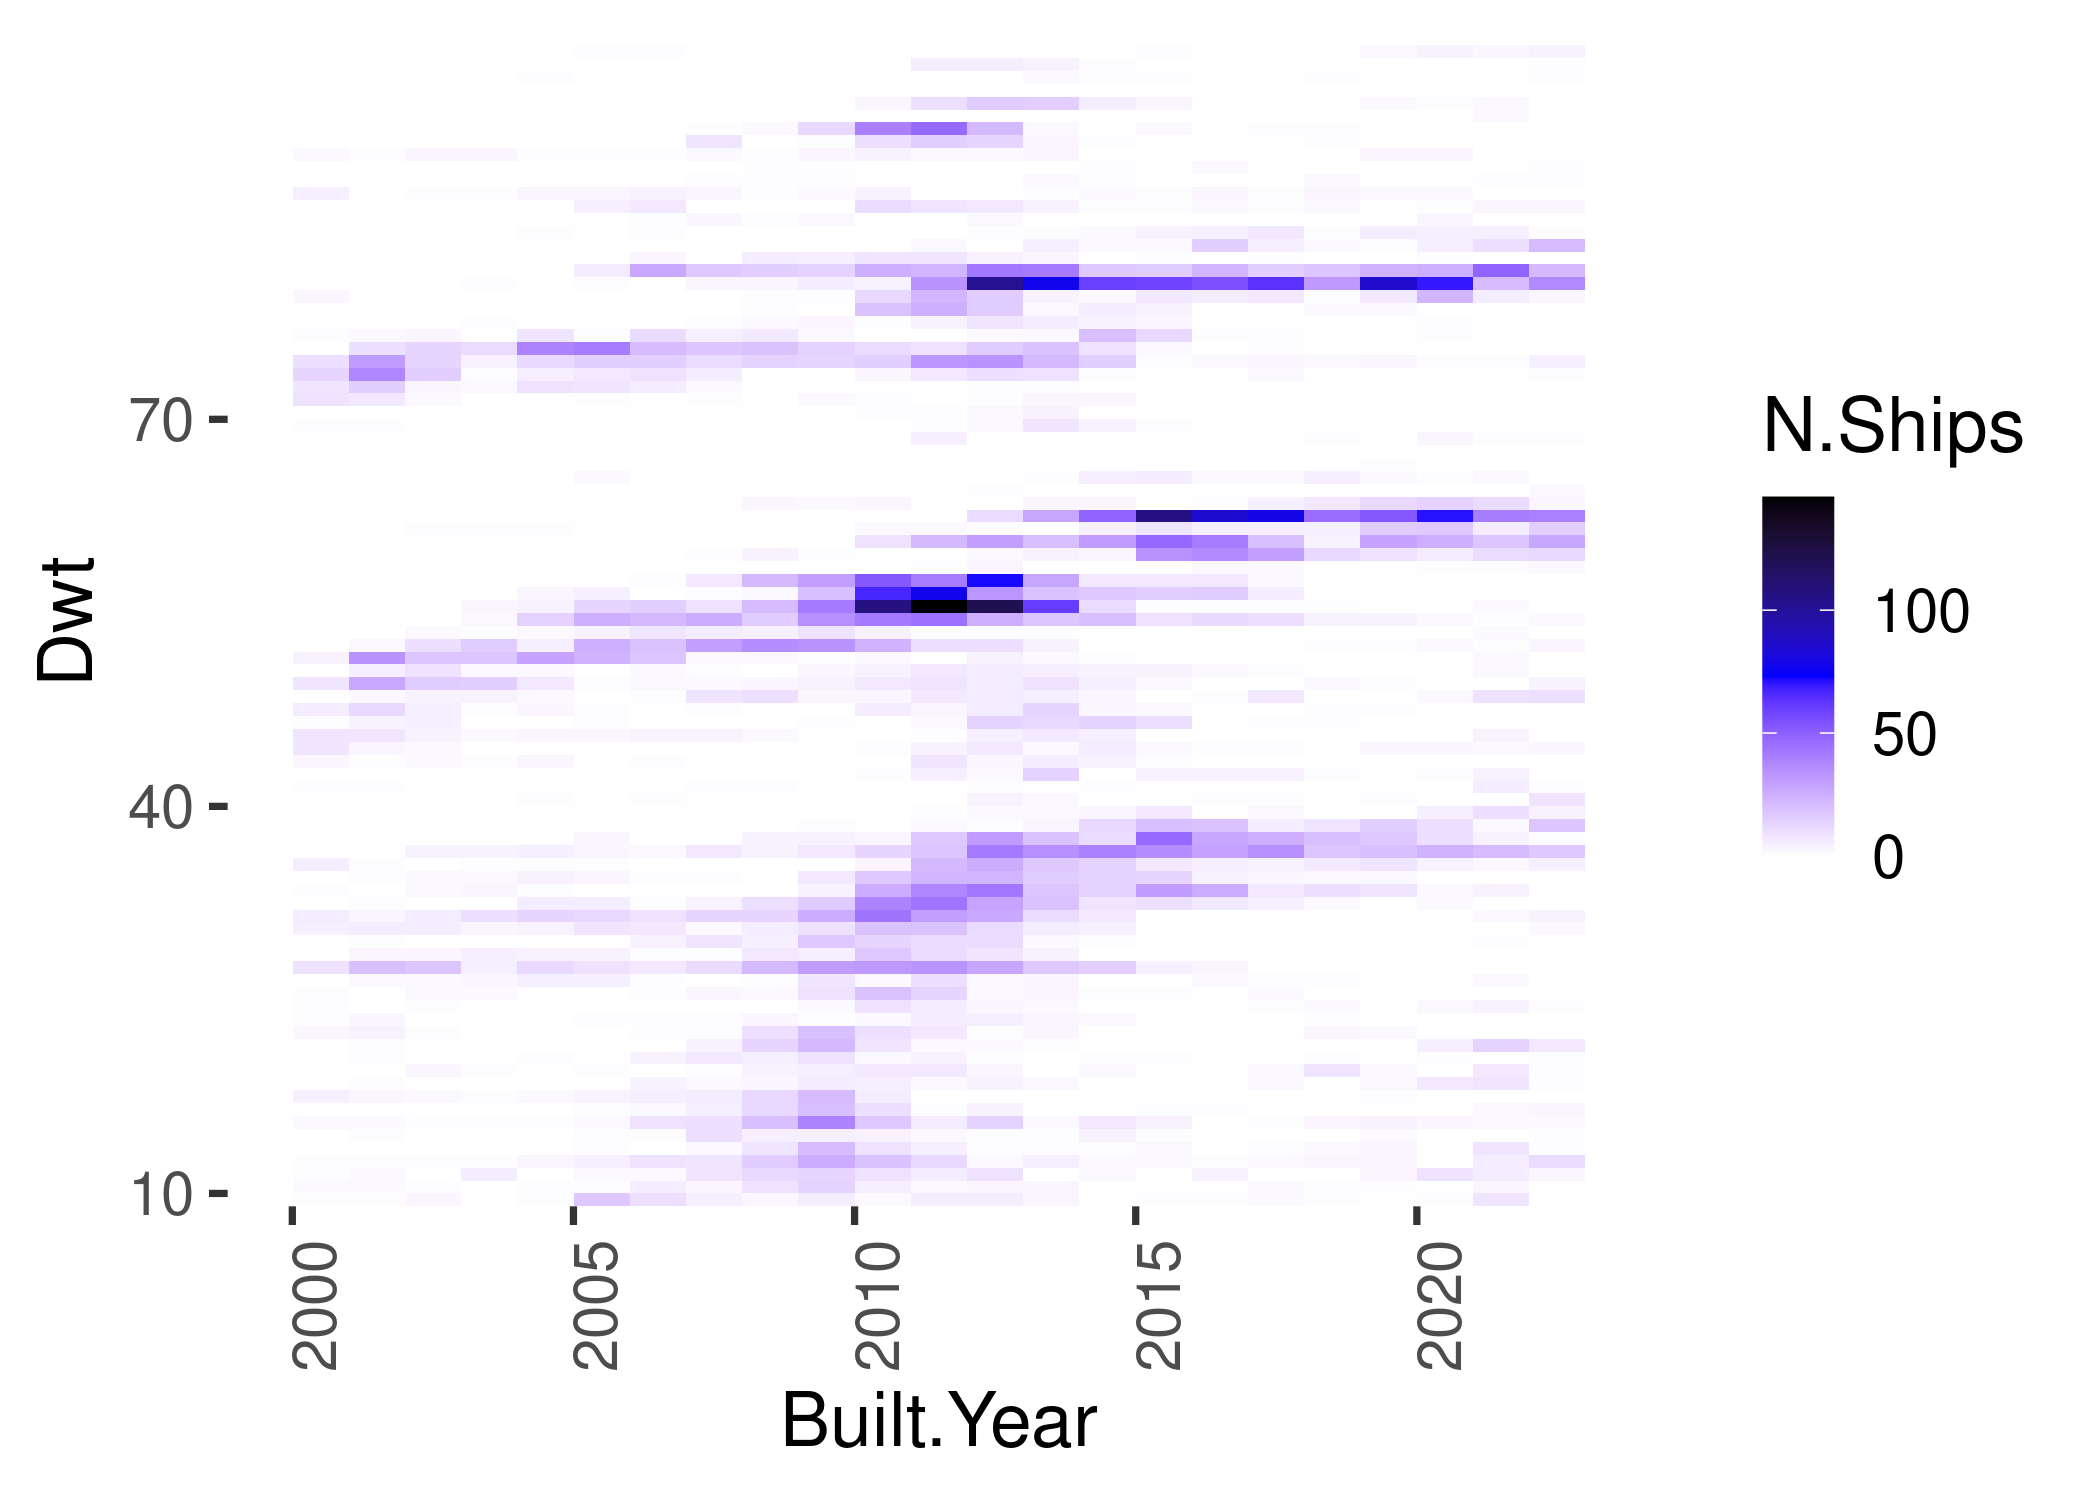
\includegraphics[width = 0.75\textwidth]{/home/apeters/Documents/PhD/ShippingEmissions/docs/images/shared/WFR_Bulkers_Exploration_Size_Built_heatmap.png}
  \caption{Number of new ships by size (Dwt) and built year}
  \label{fig:distribution}
\end{figure}

\textcolor{blue}{Is this a good figure to include? Is it better to use MRV emissions plots instead?}

Shifts in the geographic distribution of trade will further impact emissions through mechanisms such as changes in shipping distances, backhaul effects (ships travel empty on certain routes due to sector-specific trade imbalances), and economies of scale (route-specific trade volumes and port infrastructure determine the size of ships used).


\textbf{relation between target and trade}
Short-run demand shocks are important because\dots
Slow adjustment of fleet
Low level of new ship-building currently because of regulation and technology uncertainty

Emissions regulations: EEDI, EEXI, CII
Effects will 

\textbf{related literature}
The most extensive work comes from the IMO itself and other related industry organizations \citep{faber2020fourth, olmer2017greenhouse}

Other direction: elasticity of trade with respect to ship fuel costs \citep{brancaccio2018impact}

\textbf{brief use of AIS for emissions}
\citet{faber2020fourth,olmer2017greenhouse}

\citet{uge2020estimation} also link MRV data with ship activity, but seek to use it to validate reported emissions in the MRV.

\textbf{Our contributions:}
\begin{itemize}
  \item first to use actual emissions rather than theoretical
  \item apply machine learning to model ship-level emissions
  \item inform policy makers and help to assess the impacts of of incoming regulations
  \item real-time tool
  \item component to long term planning of emissions policies
  \item recent evidence based off of large fluctuation from COVID
\end{itemize}

\smallskip 

\noindent \textbf{Methodology:}  

We proceed in two stages. We first develop high-frequency disaggregated emissions estimates and then we link these to trade volumes and patterns.

\textbf{Emissions estimation}
Largely follow the bottom-up methodology developed for the Fourth IMO greenhouse gas study \citep{faber2020fourth}, also used by \citet{olmer2017greenhouse, johansson2017global, jalkanen2009modelling, van2018spatially}. This matches AIS tracking data to ship characteristics in order to estimate emissions. In order to estimate ship-level emissions, they use a simple 

however we go one step further and match it to reported annual fuel consumption data for voyages into and out of the European Union. In order to match reported fuel consumption and emissions from MRV. In this way I am able to compare the relative effects of ship size and age/vintage on reported fuel consumption rather than modelled.


1. Estimate efficiency from subset reporting to MRV

2. Extrapolate efficiencies to non-reporting ships

3. Interpolate higher frequency

4. Aggregate

\textbf{Emissions data}
We have gathered a rich set of data encompassing emissions, ship activity, fleet characteristics, and market activity

The World Fleet Register from Clarksons Research is a virtually complete listing of all large merchant ships. It includes variables such as owner, build year, ship type, and importantly for our purposes, detailed data on the technical characteristics of each ship such as dimensions, fuel type, engine type, and often even make and model of the engine. 

The AIS tracking data that contains granular information on ship movements every few minutes. We employ hourly data. This includes speed, location, and even draft, which can indicate whether it is carrying cargo or not. We will use this to construct detailed travel histories of each ship, including route, distance travelled and speed. 

Finally, publicly available data collected through the European Union's Monitoring, Reporting, and Verification (MRV) regulation provides annual fuel consumption and emissions, beginning in 2018. Tracking data can be matched at the ship-level using individual ship identifiers.

\textbf{Emissions Method}
We detect voyages from hourly ship tracking data spanning three years and encompassing essentially all dry bulk ships worldwide. We match it to reported annual fuel consumption data for voyages into and out of the European Union. 
Trip detection is validated by comparing reported distance travelled to calculated distance travelled from AIS data. 
In this way we are able to compare the relative effects of ship size and age/vintage on reported fuel consumption. 

Validate trip detection with reported distance travelled


Advantages and limitations:
Many impacts such as power curve (consumption away from design speed), hull-roughening, hull-fouling, weather are hard to predict theoretically \citep{olmer2017greenhouse}
Emisions data is annual 

weather data as per \citet{brancaccio2020geography}

\textbf{current progress}
To date, we have focused on the dry bulk industry and constructed a simple linear predictive model for efficiency estimation. 

\begin{equation}
\log\left(
    \frac{fuel~consumption}{Dwt \cdot \sum_{x \in X}  \cdot s_x^2 \cdot x}
\right)_{it}    
        = \delta age_{it} + \boldsymbol{\beta}log(Z_i) + \varepsilon_{it}
\end{equation}

As shown in \autoref{fig:efficiency}, preliminary results indicate that efficiency after controlling for size is surprisingly flat until roughly 2013 when new ship efficiency regulations were implemented. 
**compare to \citep{faber2015historical} figure 15


\begin{figure}[h]
  \centering
  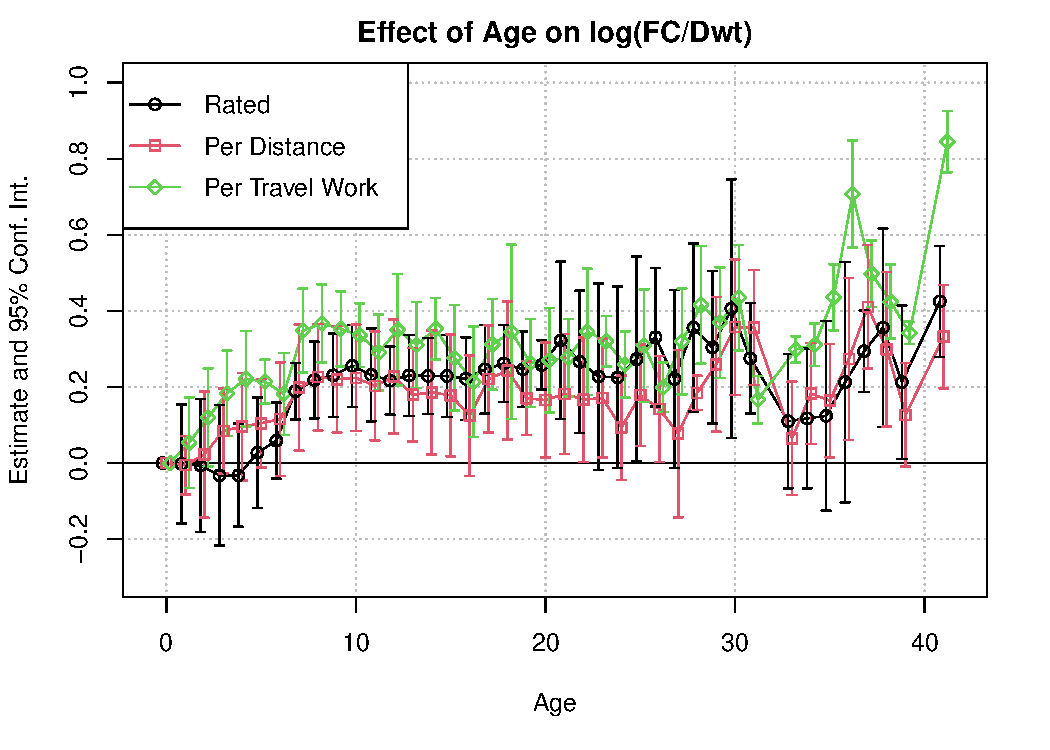
\includegraphics[width = 0.75\textwidth]{/home/apeters/Documents/PhD/ShippingEmissions/docs/images/shared/Efficiency_Regression_Size_Age_Coeffs_3.pdf}
  \caption{UPDATE THIS!}
  \label{fig:efficiency}
\end{figure}

Our next goal is to develop a more accurate neural network model. Explain neural network predictive model and training procedure
Subsequently expand to containerships

% Trade
%% Data
COVID variation
\textbf{Trade data} Bilateral trade data from...

\textbf{Method of linking to emissions to trade}
Begin with global, then incorporate geographical variation


\pagebreak
Potential data purchases:
\begin{itemize}
  \item expand time series of AIS tracking data beyond 2021
  \item AIS tracking data for tankers
  \item bilateral trade
\end{itemize}

\pagebreak
  
% \printbibliography[heading = subbibliography]
\singlespace{
\bibliography{sshrc2023shipping}
}

 

\end{document}